\documentclass[12pt]{article} % -- letter, article, report, book, memoir



\usepackage{amsmath}
\usepackage{amssymb}
\usepackage{tikz}
\usepackage{graphicx}
\usepackage{hyperref}
\usepackage{wrapfig}
\usepackage{physics}
%=====linear algebra and general math notations
\newcommand{\rr}{\mathbb{R}}
\newcommand{\zz}{\mathbb{Z}}
\newcommand{\nn}{\mathbb{N}}
\newcommand{\cc}{\mathbb{C}}
\newcommand{\re}{\mathrm{Re}}
\newcommand{\im}{\mathrm{Im}}
\newcommand{\infnorm}[1]{\norm{#1}_{\infty}}
\newcommand{\twonorm}[1]{\norm{#1}_{2}}
\newcommand{\onenorm}[1]{\norm{#1}_{1}}
\newcommand{\iprod}[1]{\langle #1 \rangle}
\newcommand{\generalmatrixA}{
	\begin{pmatrix}
		a_{11} & a_{12} & \cdots & a_{1n} \\
		a_{21} & a_{22} & \cdots & a_{2n} \\
		\vdots & \vdots & \ddots & \vdots \\
		a_{n1} & a_{n2} & \cdots & a_{nn} \\
	\end{pmatrix}
}
%=====
%===== probability theory and random processes
\newcommand{\expect}[1]{\mathbb{E}\big[ {#1} \big]}
\newcommand{\cov}[1]{\mathbb{C}ov({#1})}
\newcommand{\pp}[1]{\mathbb{P}({#1})}
\newcommand{\variance}[1]{\mathbb{V}ar\big[{#1}\big]}
%=====
%===== PDE theory
\newcommand{\intervoo}[2]{(#1, #2)}
\newcommand{\intervcc}[2]{\big[ #1, #2\big]}
\newcommand{\pdx}[1]{\frac{\partial}{\partial {#1}}}
\newcommand{\pddx}[1]{\frac{\partial^2}{\partial {#1}^2}}
\newcommand{\uno}{\large \textcircled{\small{1}}}
\newcommand{\dos}{\large\textcircled{\small{2}}}
\newcommand{\tres}{\large\textcircled{\small{3}}}
\newcommand{\yonn}{\large\textcircled{\small{4}}} % 4 in Japanese
\newcommand{\cancels}[1]{\underbrace{#1}_\textrm{cancelled}}
\newcommand{\ka}{\kappa}
\newcommand{\ga}{\gamma}
\newcommand{\uu}[2]{U_{#1}^{#2}} % shorthand
%=====
% ----------
\author{Hongli Zhao}
\title{Math 228B: Project 4 Writeup}
\date{\today}

\begin{document}
\maketitle
% ================ start file
\section{2D Poisson Problem with Homogeneous Neumann Boundary Conditions}
$$
	\begin{cases}
		-\nabla^2 u(x,y) = 1, \text{ on $\Omega$}\\
		n \cdot \nabla u = 0, \text{ on $\Gamma_1$}\\
		u = 0, \text{ on $\Gamma_2$}
	\end{cases}
$$ and the boundary is $\Gamma = \Gamma_1 \cup \Gamma_2$.

In the general case where we solve:
$$
	\begin{cases}
		-\nabla^2 u(x,y) = f \\
		n \cdot \nabla u = g
	\end{cases}
$$

First by multiplying both sides of the PDE by a test function $v\in V_h$ and integrating by parts yields:
$$
	\int_{\Omega}-\nabla^2 u_h vdx = \int_{\Omega}fv dx
$$ then applying divergence theorem and using the Neumann condition gives:
$$
	\int_{\Omega}\nabla u_n \cdot \nabla v dx = \int_{\Omega}fv dx + \oint_{\Gamma}gv ds
$$

Using $u_h(x) = \sum_{j=1}^{n}\xi_j\phi_j$ and let $v = \phi_i$:
$$
	\int_{\Omega}\bigg[ \sum_{j=1}^{n}\xi_j\nabla\phi_{j}\bigg]\cdot\nabla\phi_idx = \int_{\Omega}f\phi_idx +\oint_{\Gamma}g\phi_{i}ds
$$

Switching the order of integration and summation, we form the system:
$$
	A\xi = b
$$ where:
$$
	A_{ij} = \int_{\Omega}\nabla\phi_{i}\cdot\nabla\phi_{j}dx
$$
$$
	b_i = \int_{\Omega}f\phi_{i}dx + \oint_{\Gamma}g\phi_ids
$$

In our problem, $f = 1$ for all $\omega\in\Omega$, $g = 0$ for Neumann condition on the boundary $\Gamma$. Restricting the function to each triangle, the element stiffness matrix and load vector are given by:
$$
	a_{ij}^{K} = \int_{K}\nabla \phi_{i}\nabla\phi_{j}dx
$$
$$
	b_{i}^{K} = \int_{K}f\phi_{i}dx + \int_{K\cap\Gamma}g\phi_{i}dx = \int_{K}\phi_idx
$$

Here we derive how to compute the entries on a general triangle, using piecewise linear elements $\phi_j$. Let $K$ be described by nodes $N_1,N_2,N_3$ whose coordinates are $(x_i,y_i)$ for $i=1,2,3$. Then using the fact that $\phi_{i}(N_j)=\delta_{ij}$, we fit a linear function by solving:
$$
	\begin{cases}
		\phi_{i}(N_i) = 1 \\
		\phi_{i}(N_j) = 0 \\
		\phi_{i}(N_k) = 0 \\
	\end{cases}
$$

Let $\phi_{i} = ax + by + c$ be the general form, we plug in the coordinates and solve a system:
$$
\begin{cases}
	ax_{i}+by_{i}+c = 1 \\
	ax_{j}+by_{j}+c = 0 \\
	ax_{k}+by_{k}+c = 0 \\
\end{cases}
$$ yielding:
$$
	\begin{cases}
		a = \hat{a} = -\frac{y_k-y_j}{x_k-x_j}b\\
		b = \hat{b} = \frac{1}{y_i-y_j} + \frac{(x_i-x_j)(y_k-y_j)}{(y_i-y_j)(x_k-x_j)} \\
		c = \hat{c} = 1-x_ia - y_ib
	\end{cases}
$$

Knowing explicitly what $\hat{a},\hat{b},\hat{c}$ are, we can get explicitly the piecewise linear functions:
$$
	\phi_i(x,y) = a_ix+b_iy+c_i
$$

Then:
$$
	\nabla \phi_{i} = a_i + b_i
$$

For the local stiffness matrix, we can compute the entries explicitly:
$$
	a_{ij}^{K} = \int_{K}\nabla\phi_{i}\nabla\phi_{j}dx = \big[(a_i \cdot a_j)+(b_i \cdot b_j)\big]\cdot \text{ (Area of $K$) }
$$ where $a_i,a_j,b_i,b_j$ are coefficients of the basis functions. Given that we know the coordinates for each triangle $K$, the area can easily be computed by using the system matrix:
$$
	B = 
	\begin{pmatrix}
		x_i & y_i & 1 \\
		x_j & y_j & 1 \\
		x_k & y_k & 1
	\end{pmatrix}
$$ then we have $\det B = 2\cdot(\text{ Area of K } )$, or $(\text{ Area of K }) = \frac12 \det B$.

For the load vector:
$$
	b_i = \int_{K} \phi_i dx
$$ this corresponds to the volume under our piecewise linear "plane", over the triangular area $K$, this corresponds to $\frac13$ of the volume of the prism with unit height, or:
$$
	b_i = \frac13\cdot (\text{ Area of $K$ } \cdot 1) = \frac16 \det B
$$

Now that we have explicitly the entries of $A$ and load vector $b$, we can assemble the global stiffness matrix using the stamping method.

After we have computed the global system vector $\xi$ for the Neumann problem, we can then impose the Dirichlet data by directly replacing the $\xi$'s for nodes that are on the Dirichlet boundary.

Since the nodal basis function can unique determine our numerical solution, the computed solutions at each nodal points are:
$$
	u_h(N_i) = \xi_i
$$ where $\xi_i$ are the entries that we computed from the stiffness matrix.

\subsection{result presentation}
Running the script:
\begin{verbatim}
	\ fempoitst.m
\end{verbatim} provides 3 outputs as follows:

\begin{figure}[h!]
 \centering
 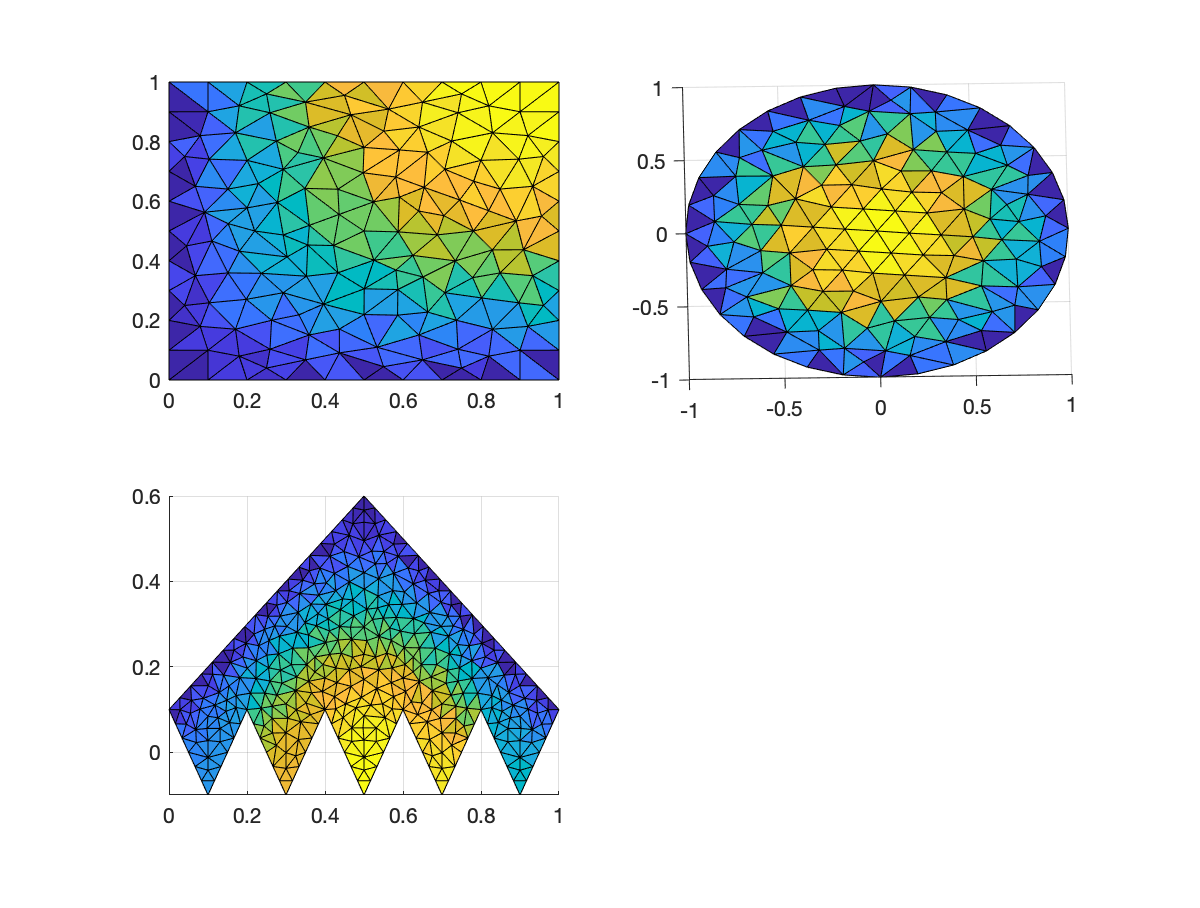
\includegraphics[width=0.8\textwidth]{result1-2d.eps}
 \caption{2D color surface plot of results}
\end{figure}
\begin{figure}[h!]
\centering
 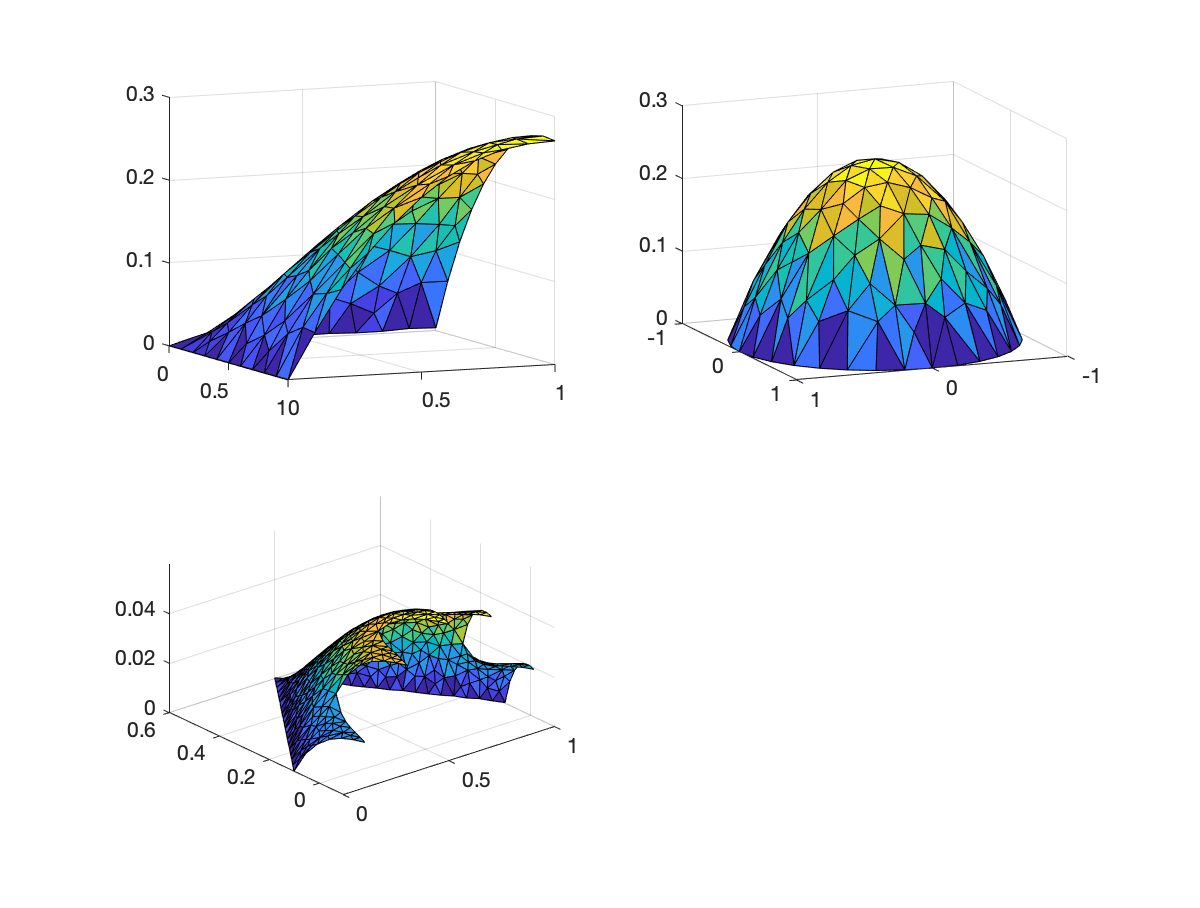
\includegraphics[width=0.8\textwidth]{result1-3d.eps}
 \caption{3D color surface plot of results}
\end{figure}

Achieved in fempoi.m by solving with homogeneous Neumann condition first and replacing with Dirichlet conditions for mixed boundary porblems.
\newpage

\section{Errors for All-Dirichlet Problem}
Using the
\begin{verbatim}
	fempoi.m
\end{verbatim} routine defined from part 1, we solve two Poisson problems using all-Dirichlet conditions on a square mesh and a polygon mesh. Using the finest level of refinement as an exact solution, we take max norm at each step and plot the log-log error behaviors. The error plot is presented as follows; we see that our convergence rate is roughly better than second order.
\begin{figure}[h!]
 \centering
 \includegraphics[width=0.8\textwidth]{convergence.eps}
 \caption{Error behaviors for two meshes, Poisson Problem 2D}
\end{figure}

\newpage
Obtained through running the script:
\begin{verbatim}
	poiconvtst.m
\end{verbatim}, which also provides the error and rate information as follows:
\begin{verbatim}
>> poiconvtst
% solving square mesh problem
errors =

    0.0279
    0.0073
    0.0015

displaying the convergence rate ...
====================

rate =

    2.3164

% solving polygon mesh problem
errors =

    0.0495
    0.0118
    0.0024

displaying the convergence rate ...
====================

rate =

    2.3219

>> 
\end{verbatim}


\section{Fourth Order Boundary Value Problem}
\subsection{Galerkin Formulation}
We would like to find $u_h\in V_h$ such that:
$$
	\int_{0}^{1}u''_h(x)v''(x)dx = \int_0^{1}f(x)v(x) dx
$$

The Galerkin formulation is derived by using an appropriate functional space for $v\in V_h$ (keeping the boundary conditions $v(0)=v(1)=v'(0) = v'(1) = 0$) and applying integration by parts two times.

Starting from the PDE:
$$
	u''''(x) = f(x)
$$ 

Multiply both sides by test function $v(x) \in V_h$, and integrate across the domain:
$$
	u''''(x) v(x) = f(x)v(x)
$$
$$
	\int_{0}^{1} u''''(x) v(x)dx
	=
	\int_{0}^{1}f(x)v(x)dx
$$

Let $u = v(x)$, $dv = u''''(x)dx$, we can integrate the left hand side of the PDE by parts.
$$
	\int_{0}^{1} u''''(x) v(x)dx = v(x)u'''(x)\biggr\rvert_{0}^{1} - \int_0^1 u'''(x)v'(x)dx
$$

Since $v(0) = v(1) = 0$, we have:
$$
	\int_{0}^{1} u''''(x) v(x)dx
	=
	-\int_0^1 u'''(x)v'(x)dx
$$

Now we need to integrate the new expression by parts, let $u = v'(x)$, $dv = u'''(x)dx$, we apply integration by parts again:
$$
	-(\int_0^1 u'''(x)v'(x)dx)
=
-(v'(x)u''(x)\biggr\rvert_{0}^1 - \int_0^1 u''(x)v''(x)dx)
$$ but $v'(0)=v'(1) = 0$ by our formulation, then we have finally the LHS:
$$
	\int_{0}^{1} u''''(x) v(x)dx = - (-\int_0^1 u''(x)v''(x)dx) = \int_0^1 u''(x)v''(x)dx
$$

which gives us the Galerkin formulation:

Find $u = u_h$ such that:
$$
	(u_h'',v'') = (f,v)
$$ holds for all $v\in V_h$, or explicitly
$$
	\int_0^1 u_h''(x)v''(x)dx
	=
	\int_0^1 f(x)v(x)dx
$$

\subsection{Hermite Bases}
In each element $K_1, K_2$, we would like to have a degree 3 polynomial, and the overall basis function $\phi_1$ and $\phi_2\in V_h$ should match the values at 0 and 1 as well as their derivatives. Additionally, we also need the polynomial $\phi_i$ to have continuity for both itself and its first order derivative. 

Since in each $K_i, i= 1,2$, we would need a degree-3 polynomial, we would have 4 degrees of freedom in that element, and 8 degrees of freedom for $\phi_i$ overall. Since we require $\phi(0)=\phi'(0)=\phi(1)=\phi'(1) = 0$, and continuity at both $\phi(\frac12),\phi'(\frac12)$, we have that:
$$
	\dim V_h = 8 - 4 - 2 = 2
$$ which means our functional basis has 2 degrees of freedom.

Define $\phi_1(x)\in V_h$ with the following conditions:
$$
	\begin{cases}
		\phi_1(0) = \phi_1'(0) = 0\\
		\phi_1(\frac12) = 0\\
		\phi_1'(\frac12) = 1\\
		\phi_{1}(1) = \phi_1'(1) = 0	
	\end{cases}
$$

Let $\phi_1(x) = a_1x^3 + b_1x^2 + c_1x + d_1$ in $K_1$ and $\phi_1(x) = a_2x^3 + b_2x^2 + c_2x + d_2$ in $K_2$, and we have the system for its coefficients:
$$
	\begin{cases}
		d_1 = 0\\
		c_1 = 0\\
		\frac18 a_1 + \frac14 b_1 + \frac12 c_1 + d_1 = 0\\
		\frac34 a_1 + b_1 + c_1 = 1
	\end{cases}
$$

Giving us the coefficients:
$$
	\begin{cases}
		a_1 = 4\\
		b_1 = -2\\
		c_1 = 0\\
		d_1 = 0
	\end{cases}
$$

Similarly in $K_2$:
$$
	\begin{cases}
		\frac18 a_2 + \frac14 b_2 + \frac12 c_2 + d_2 = 0 \\
		\frac34 a_2 + b_2 + c_2 = 1 \\
		a_2 + b_2 + c_2 + d_2 = 0\\
		3a_2 + 2b_2 + c_2 = 0
	\end{cases}
$$

$$
	\begin{cases}
		a_2 = 4\\
		b_2= -10\\
		c_2 = 8\\
		d_2 = -2
	\end{cases}
$$

Then we have:
$$
	\phi_1(x) = 
	\begin{cases}
		4x^3 - 2x^2, \text{ $x \in K_1$}\\
		4x^3 -10x^2 + 8x - 2, \text{ $x\in K_2$}
	\end{cases}
$$

Similarly, we can define $\phi_2(x)\in V_h$ with the following conditions, altering the behavior at $\phi_2(\frac12)$ as long as it is different from $\phi_1$.
$$
	\begin{cases}
		\phi_2(0) = \phi_2'(0) = 0\\
		\phi_2(\frac12) = 1\\
		\phi_2'(\frac12) = 1\\
		\phi_{2}(1) = \phi_2'(1) = 0	
	\end{cases}
$$

Let $\phi_2(x) = a_1'x^3 + b_1'x^2 + c_1'x + d_1'$ in $K_1$ and $\phi_2(x) = a_2'x^3 + b_2'x^2 + c_2'x + d_2'$ in $K_2$, and we have the system for its coefficients:
$$
	\begin{cases}
		d_1' = 0\\
		c_1' = 0\\
		\frac18 a_1' + \frac14 b_1' + \frac12 c_1' + d_1' = 1\\
		\frac34 a_1' + b_1' + c_1' = 1
	\end{cases}
$$

Giving us the coefficients:
$$
	\begin{cases}
		a_1' = -12\\
		b_1' = 10\\
		c_1' = 0\\
		d_1' = 0
	\end{cases}
$$

In $K_2$:
$$
	\begin{cases}
		\frac18 a_2' + \frac14 b_2' + \frac12 c_2' + d_2' = 1 \\
		\frac34 a_2' + b_2' + c_2' = 1 \\
		a_2' + b_2' + c_2' + d_2' = 0\\
		3a_2' + 2b_2' + c_2' = 0
	\end{cases}
$$

$$
	\begin{cases}
		a_2' = 20\\
		b_2'= -46\\
		c_2' = 32\\
		d_2' = -6
	\end{cases}
$$

Then we have:
$$
	\phi_2(x) = 
	\begin{cases}
		-12x^3 + 10x^2, \text{ $x \in K_1$}\\
		20x^3 -46x^2 + 32x - 6, \text{ $x\in K_2$}
	\end{cases}
$$


Therefore $\{\phi_1,\phi_2\}$ can serve as one basis for $V_h$.


\subsection{Numerical solution}
The exact solution is given by:
$$
	u^{(4)}(x) = 480x-120
$$
$$
	u'''(x) = 240x^2 - 120x +c_1
$$
$$
	u''(x) = 80x^3 - 60x^2 + c_1x + c_2
$$
$$
	u'(x) = 20x^4 - 20x^3 + \frac12 c_1x^2 + c_2x + c_3
$$
$$
	u(x) = 4x^5 - 5x^4 + \frac16 c_1x^3 + \frac12 c_2x^2 + c_3x + c_4
$$

Then plugging in the boundary conditions would give us:
$$
	u(0) = u(1) = u'(0) = u'(1) = 0
$$

$$
	\begin{cases}
		c_4 = 0 \\
		4-5+\frac16 c_1 + \frac12 c_2 + c_3 +c_4= 0\\
		c_3 = 0 \\
		20 - 20 + \frac12c_1 + c_2 + c_3 = 0
	\end{cases}
$$ solve, and we have:
$$
	\begin{cases}
		c_1 = -12\\
		c_2 = 6\\
		c_3 = c_4 = 0
	\end{cases}
$$ thus the final exact solution is given by:
$$
	u_{exact}(x) = 4x^5 - 5x^4 - 2x^3 + 3x^2
$$ we can verify:
$$
	u'''' = 4 \cdot (5\cdot 4\cdot 3\cdot 2)x - 5! = 480x - 120
$$


Using the basis defined above, we test the numerical solution. First we begin by assembling the stiffness matrix and load vector.

Let $u_h = \xi_1\phi_1 + \xi_2\phi_2$. We would like to solve for the $\xi$ vector.

Using the variational formulation, let $v(x) = \phi_j(x)$:
$$
	LHS = \int_0^1 u''_h(x)v''(x)dx
	= \int_0^1 \sum_{i=1}^{2}\xi_i\phi''_i(x) \phi_j''(x)dx
$$
$$
	= \sum_{i=1}^{2}\xi_i\int_{0}^{1}\phi_i''(x)\phi_j''(x)dx = \sum_{i=1}^{2}\xi_ia_{ij}
$$ where $a_{ij} = \int\phi_i''\phi_j''dx$.

The load vector is:
$$
	RHS = \int_0^1f(x)v(x)dx
	= \int_{0}^{1}f(x)\phi_j(x)dx = b_j
$$

Then concisely:
$$
	\sum_{i=1}^{2}\xi_ia_{ij} = b_j
$$
$$
	A\xi = b
$$ where $A\in\rr^{2\times 2}$. 

Due to our functional space being small, we can explicitly calculate the stiffness matrix and load vector, which we do so in the numerical implementation. The main routine is presented in:
\begin{verbatim}
prob3_beam.m
\end{verbatim} which uses MATLAB symbolic computation to explicitly compute the functions composed of the functional basis $\phi_i\in V_h$, and then calculate our desired integrals.

The result is presented below:
\begin{figure}[h!]
\centering
 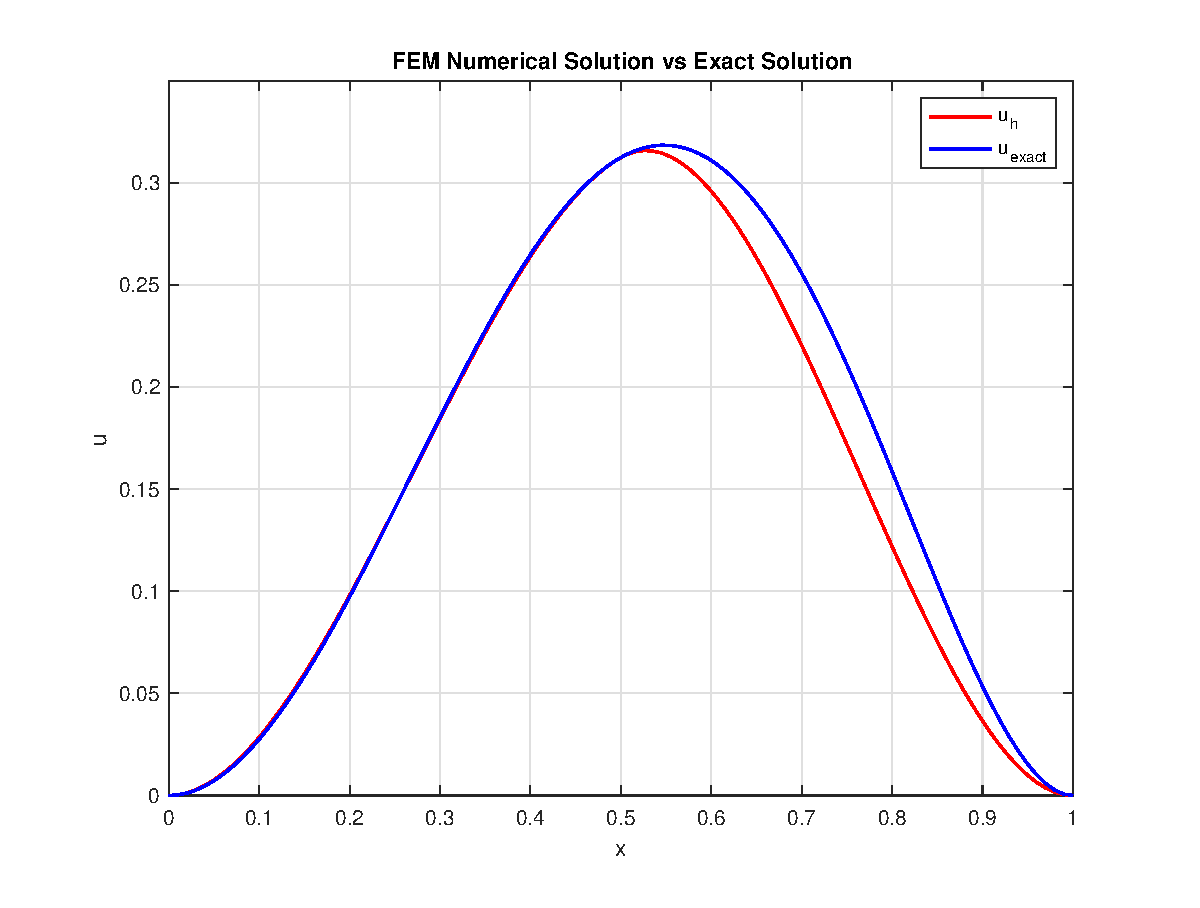
\includegraphics[width=0.8\textwidth]{p3_numerical.eps}
 \caption{Numerical Solution versus Exact Solution for $u(x)$}
\end{figure}

\newpage
We see that our FEM formulation with this $V_h$ is able to capture the exact solution relatively well except for the second half. If we: 
\newline
(1) analytically integrate all integrals (to avoid numerical errors) and
\newline
(2) increase the number of elements, 
\
\newline
we should expect better convergence.


% ================ end file
\end{document}

